%%%%%%%%%%%%%%%%%%%% author.tex %%%%%%%%%%%%%%%%%%%%%%%%%%%%%%%%%%%
%
% sample root file for your "contribution" to a contributed volume
%
% Use this file as a template for your own input.
%
%%%%%%%%%%%%%%%% Springer %%%%%%%%%%%%%%%%%%%%%%%%%%%%%%%%%%


% RECOMMENDED %%%%%%%%%%%%%%%%%%%%%%%%%%%%%%%%%%%%%%%%%%%%%%%%%%%
\documentclass[graybox]{svmult}

% choose options for [] as required from the list
% in the Reference Guide

\usepackage{mathptmx}       % selects Times Roman as basic font
\usepackage{helvet}         % selects Helvetica as sans-serif font
\usepackage{courier}        % selects Courier as typewriter font
\usepackage{type1cm}        % activate if the above 3 fonts are
                            % not available on your system
%
\usepackage{makeidx}         % allows index generation
\usepackage{graphicx}        % standard LaTeX graphics tool
                             % when including figure files
\usepackage{multicol}        % used for the two-column index
\usepackage[bottom]{footmisc}% places footnotes at page bottom

% see the list of further useful packages
% in the Reference Guide

\usepackage[]{amssymb, amsmath}
\usepackage[]{bm}
\usepackage[]{upgreek}
\usepackage[]{graphicx}

\DeclareMathAlphabet{\mathcal}{OMS}{cmsy}{m}{n}
\DeclareMathAlphabet\mathbfcal{OMS}{cmsy}{b}{n}
\graphicspath{{imgs/}}

\makeindex             % used for the subject index
                       % please use the style svind.ist with
                       % your makeindex program

%%%%%%%%%%%%%%%%%%%%%%%%%%%%%%%%%%%%%%%%%%%%%%%%%%%%%%%%%%%%%%%%%%%%%%%%%%%%%%%%%%%%%%%%%

\begin{document}

\title*{Time-stepping and Krylov methods for large-scale instability problems}
% Use \titlerunning{Short Title} for an abbreviated version of
% your contribution title if the original one is too long
\author{J.-Ch. Loiseau \and M. A. Bucci \and S. Cherubini \and J.-Ch. Robinet}
% Use \authorrunning{Short Title} for an abbreviated version of
% your contribution title if the original one is too long
\institute{J.-Ch. Loiseau \at Laboratoire DynFluid, Arts et M\'etiers ParisTech, 151 boulevard de l'h\^opital, 75013 Paris, France. \email{jean-christophe.loiseau@ensam.eu}
\and M. A. Bucci \at  Laboratoire DynFluid, Arts et M\'etiers ParisTech, 151 boulevard de l'h\^opital, 75013 Paris, France. \email{michele.bucci@ensam.eu}
\and S. Cherubini \at DMMM, Politecnico di Bari, via Re David 200, 70100 Bari, Italy. \email{s.cherubini@gmail.com}
\and J.-Ch. Robinet \at  Laboratoire DynFluid, Arts et M\'etiers ParisTech, 151 boulevard de l'h\^opital, 75013 Paris, France. \email{jean-christophe.robinet@ensam.eu}}
%
% Use the package "url.sty" to avoid
% problems with special characters
% used in your e-mail or web address
%
\maketitle

%%%%%%%%%%%%%%%%%%%%%%%%%%%%
%%%%%                  %%%%%
%%%%%     ABSTRACT     %%%%%
%%%%%                  %%%%%
%%%%%%%%%%%%%%%%%%%%%%%%%%%%

\abstract*{???}

\abstract{???}


%%%%%%%%%%%%%%%%%%%%%%%%%%%%%%%%%%%%%
%%%%%                           %%%%%
%%%%%     COEUR DU CHAPITRE     %%%%%
%%%%%                           %%%%%
%%%%%%%%%%%%%%%%%%%%%%%%%%%%%%%%%%%%%

% --> Introduction.
\section{Introduction}
\label{sec: introduction}


% --> Theoretical framework.
\section{Theoretical framework}
\label{sec: theory}

  Our attention is focused on the characterization of very high-dimensional nonlinear dynamical systems typically arising from the spatial discretization of partial differential equations such as the incompressible Navier-Stokes equations. In general, the resulting dynamical equations are written down as a system of first order differential equations
  \begin{equation}
    \dot{X}_j = \mathcal{F}_j \left( \left\{ X_i(t);\ i =1, \cdots, n \right\}, t \right)
    \notag
  \end{equation}
  where the integer $n$ is the \emph{dimension} of the system, and $\dot{X}_j$ denotes the time-derivative of $X_j$. Using the notation $\bf{X}$ and $\mathbfcal{F}$ for the sets $\left\{ X_j,\ i =1, \cdots, n \right\}$ and $\left\{ \mathcal{F}_j,\ i =1, \cdots, n \right\}$, this system can be compactly written as
  \begin{equation}
    \dot{\mathbf{X}} = \mathbfcal{F}(\mathbf{X}, t),
    \label{eq: theory -- continuous-time dynamical system}
  \end{equation}
  where $\mathbf{X}$ is the $n \times 1$ \emph{state vector} of the system and $t$ is a continuous variable denoting time. Alternatively, accounting also for temporal discretization gives rise to a discrete-time dynamical system
  \begin{equation}
    X_{j, k+1} = \Phi_j \left( \left\{ X_{i, k};\ i = 1, \cdots, n \right\}, k \right)
    \notag
  \end{equation}
  or formally
  \begin{equation}
    \mathbf{X}_{k+1} = \bm{\Phi}(\mathbf{X}_k, k)
    \label{eq: theory -- discrete-time dynamical system}
  \end{equation}
  where the index $k$ now denotes the discrete time variable. If one uses first-order Euler extrapolation for the time discretization, the relation between $\mathbfcal{F}$ and $\bm{\Phi}$ is given by
  \begin{equation}
    \bm{\Phi}(\mathbf{X}) = \mathbf{X} + \Updelta t \mathbfcal{F}\left( \mathbf{X} \right),
    \notag
  \end{equation}
  where $\Updelta t$ is the time-step and the explicit dependences on $t$ and $k$ have been dropped for the sake of simplicity.

  In the rest of this section, the reader will be introduced to the concepts of fixed points and linear stability, two concepts required to characterize a number of properties of the system investigated. Particular attention will be paid to \emph{modal} and \emph{non-modal stability}, two approaches that have become increasingly popular in fluid dynamics over the past decades. Note that the concept of \emph{nonlinear optimal perturbation}, which has raised a lot attention lately, is beyond the scope of the present contribution. For interested readers, please refer to the recent work by \cite{nonlinear_optimal:kerswell:2014} and references therein.

  Finally, while we will mostly use the continuous-time representation \eqref{eq: theory -- continuous-time dynamical system} when introducing the reader to the theoretical concepts exposed in this section, using the discrete-time representation \eqref{eq: theory -- discrete-time dynamical system} will prove more useful when discussing and implementing the different algorithms presented in \textsection \ref{sec: numerics}.


  %%%%%%%%%%%%%%%%%%%%%%%%%%%%%%%%
  %%%%%                      %%%%%
  %%%%%     FIXED POINTS     %%%%%
  %%%%%                      %%%%%
  %%%%%%%%%%%%%%%%%%%%%%%%%%%%%%%%

  \subsection{Fixed points}
  \label{subsec: theory-fixed points}

  Nonlinear dynamical systems described by Eq.~\eqref{eq: theory -- continuous-time dynamical system} or Eq.~\eqref{eq: theory -- discrete-time dynamical system} tend to admit a number of different equilibria forming the backbone of their phase space. These different equilibria can take the form of fixed points, periodic orbits or strange attractors for instance. In the rest of this work, our attention will be solely focused on fixed points.

  For a continuous-time dynamical system described by Eq.~\eqref{eq: theory -- continuous-time dynamical system}, fixed points $\mathbf{X}^{*}$ are solution to
  \begin{equation}
    \mathbfcal{F}\left( \mathbf{X} \right) = 0.
    \label{eq: theory -- continuous-time fixed point}
  \end{equation}
  Conversely, fixed points $\mathbf{X}^*$ of a discrete-time dynamical system described by Eq.~\eqref{eq: theory -- discrete-time dynamical system} are solution to
  \begin{equation}
    \bm{\Phi} \left( \mathbf{X} \right) = \mathbf{X}.
    \label{eq: theory -- discrete-time fixed point}
  \end{equation}
  It must be emphasized that both Eq.~\eqref{eq: theory -- continuous-time fixed point} and Eq.~\eqref{eq: theory -- discrete-time fixed point} may admit multiple solutions. Such a multiplicity of fixed points can easily be illustrated by a simple Duffing oscillator given by
  \begin{equation}
    \begin{aligned}
      \dot{x} & = y \\
      \dot{y} & = -\displaystyle \frac{1}{2} y + x - x^3.
    \end{aligned}
    \label{eq: theory -- Duffing oscillator}
  \end{equation}
  Despite its apparent simplicity, this Duffing oscillator admits three fixed points, namely
  \begin{itemize}
    \item a saddle at the origin $\mathbf{X}^* = (0, 0)$,
    \item two linearly stable spirals located at $\mathbf{X}^* = (\pm 1, 0)$.
  \end{itemize}
  All of these fixed points, along with some trajectories, are depicted on figure \ref{fig: theory -- Duffing oscillator} for the sake of illustration. Such a multiplicity of fixed points also occurs in dynamical systems as complex as the Navier-Stokes equations. Determining which of these fixed points is the most relevant one from a physical point of view is problem-dependent and left for the user to decide. Note however that computing these equilibrium points is a prerequisite to all of the analyses to be described in this chapter. Numerical methods to solve Eq.~\eqref{eq: theory -- continuous-time fixed point} or Eq.~\eqref{eq: theory -- discrete-time fixed point} will be discussed in \textsection \ref{subsec: numerics-fixed points computation}.

  \begin{figure}[b]
    \centering
    \sidecaption
    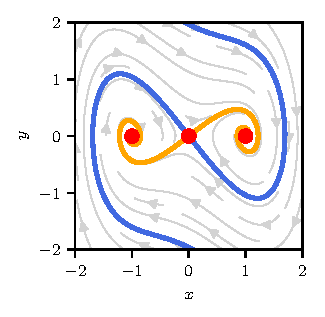
\includegraphics[scale=1]{duffing_oscillator_saddle_manifold}
    \caption{Phase portrait of the unforced Duffing oscillator \eqref{eq: theory -- Duffing oscillator}. The red dots denote the three fixed points admitted by the system. The blue (resp. orange) thick line depicts the stable (resp. unstable) manifold of the saddle point located at the origin. Grey lines highlight a few trajectories exhibited for different initial conditions.}
    \label{fig: theory -- Duffing oscillator}
  \end{figure}

  %%%%%%%%%%%%%%%%%%%%%%%%%%%%%%%%%%%%
  %%%%%                          %%%%%
  %%%%%     LINEAR STABILITY     %%%%%
  %%%%%                          %%%%%
  %%%%%%%%%%%%%%%%%%%%%%%%%%%%%%%%%%%%

  \subsection{Linear stability analysis}
  \label{subsec: theory -- linear stability}

  Having computed a given fixed point $\mathbf{X}^*$ of a continuous-time nonlinear dynamical system given by Eq. \eqref{eq: theory -- continuous-time dynamical system}, one may ask whether it corresponds to a stable or unstable equilibrium of the system. Before pursuing, the very notion of \emph{stability} needs to be explained. It is traditionally defined following the concept of Lyapunov stability. Having computed the equilibrium state $\mathbf{X}^*$, the system is perturbed around this state. If it returns back to the equilibrium point, the latter is deemed stable, otherwise, it is regarded as unstable. It has to be noted that, in the concept of Lyapunov stability, an infinite time horizon is allowed for the return to equilibrium.

  The dynamics of a perturbation $\mathbf{x} = \mathbf{X} - \mathbf{X}^*$ are governed by
  \begin{equation}
    \dot{\mathbf{x}} = \mathbfcal{F}(\mathbf{X}^* + \mathbf{x}).
  \end{equation}
  Assuming the perturbation $\mathbf{x}$ is infinitesimal, $\mathbfcal{F}(\mathbf{X})$ can be approximated by its first-order Taylor expansion around $\mathbf{X} = \mathbf{X}^*$. Doing so, the governing equations for the perturbation $\mathbf{x}$ simplify to
  \begin{equation}
    \dot{\mathbf{x}} = \mathbfcal{A}\mathbf{x},
    \label{eq: theory -- linear perturbation dynamics}
  \end{equation}
  where $\mathbfcal{A}$ is the $n \times n$ Jacobian matrix of $\mathbfcal{F}$. Starting from an initial condition $\mathbf{x}_0$, the perturbation at time $t$ is given by
  \begin{equation}
    \mathbf{x}(t) = \exp \left( \mathbfcal{A}t \right) \mathbf{x}_0.
    \label{eq: theory -- linear stability solution}
  \end{equation}
  The operator $\mathbfcal{M}(t) = \exp \left( \mathbfcal{A}t \right)$ is known as the \emph{exponential propagator}. Introducing the spectral decomposition of $\mathbfcal{A}$
  \begin{equation}
    \mathbfcal{A} = \mathbfcal{V} \boldsymbol{\Lambda} \mathbfcal{V}^{-1},
    \notag
  \end{equation}
  Eq. \eqref{eq: theory -- linear stability solution} can be rewritten as
  \begin{equation}
    \mathbf{x}(t) = \mathbfcal{V} \exp \left( \boldsymbol{\Lambda} t \right) \mathbfcal{V}^{-1} \mathbf{x}_0,
  \end{equation}
  where the i\textsuperscript{th} column of $\mathbfcal{V}$ is the eigenvector $\mathbf{v}_i$ associated to the i\textsuperscript{th} eigenvalue $\lambda_i = \boldsymbol{\Lambda}_{ii}$, with $\boldsymbol{\Lambda}$ a diagonal matrix. Assuming that the eigenvalues of $\mathbfcal{A}$ have been sorted by decreasing real part, it can easily be shown that
  \begin{equation}
    \lim\limits_{t \to + \infty} \exp \left( \mathbfcal{A} t \right) \mathbf{x}_0 = \lim \limits_{t \to + \infty} \exp \left( \lambda_1 t \right) \mathbf{v}_1 .
    \notag
  \end{equation}
  The asymptotic fate of an initial perturbation $\mathbf{x}_0$ is thus entirely dictated by the real part of the leading eigenvalue $\lambda_1$:
  \begin{itemize}
    \item if $\Re \left( \lambda_1 \right) > 0$, a random initial perturbation $\mathbf{x}_0$ will eventually grow exponentially rapidly. Hence, the fixed point $\mathbf{X}^*$ is deemed \emph{linearly unstable}.

    \item If $\Re \left( \lambda_1 \right) < 0$, the initial perturbation $\mathbf{x}_0$ will eventually decay exponentially rapidly. The fixed point $\mathbf{X}^*$ is thus \emph{linearly stable}.
  \end{itemize}
  The case $\Re \left( \lambda_1 \right) = 0$ is peculiar. The fixed point $\mathbf{X}^*$ is called \emph{elliptic} and one cannot conclude about its stability solely by looking at the eigenvalues of $\mathbfcal{A}$. In this case, one needs to resort to \emph{weakly non-linear analysis} which essentially looks at the properties of higher-order Taylor expansion of $\mathbfcal{F} \left( \mathbf{X} \right)$. Once again, this is beyond the scope of the present chapter. Interested readers are referred to \cite{??} for more details about such analyses.

  \paragraph*{Illustration}

  Let us illustrate the notion of linear stability on a simple example. For that purpose, we will consider the same linear dynamical system as in \cite{amr:schmid:2014}. This system reads
  \begin{equation}
    \displaystyle \frac{\mathrm{d}}{\mathrm{d}t} \begin{bmatrix} x_1 \\ x_2 \end{bmatrix} =
    \underbrace{
    \begin{bmatrix}
      \displaystyle \frac{1}{100} - \frac{1}{Re} & 0 \\
      1 & \displaystyle -\frac{2}{Re}
    \end{bmatrix}
    }_{\mathbfcal{A}}
    \begin{bmatrix} x_1 \\ x_2 \end{bmatrix}
    \label{eq: theory -- schmid system}
  \end{equation}
  where $Re$ is a control parameter. For such a simple case, it is obvious that the eigenvalues of $\mathbfcal{A}$ are given by
  \begin{equation}
    \lambda_1 = \displaystyle \frac{1}{100} - \frac{1}{Re}
    \notag
  \end{equation}
  and
  \begin{equation}
    \lambda_2 = - \frac{2}{Re}.
    \notag
  \end{equation}
  While $\lambda_2$ is constantly negative, $\lambda_1$ is negative for $Re < 100$ and positive otherwise. Figure \ref{fig: theory -- illustration modal stability} depicts the time-evolution of $\| \mathbf{x} \|_2^2 = x_1^2 + x_2^2$ for two different values of $Re$. Please note that the short-time ($t < 100$) behavior of the perturbation will be discussed in \textsection \ref{subsec: theory -- non-modal stability}. It is clear nonetheless that, for $t>100$, the time-evolution of the perturbation can be described by an exponential function. Whether this exponential increases or decreases as a function of time is solely dictated by the sign of $\lambda_1$, negative for $Re=50$ and positive for $Re=100$. For $Re=50$, the equilibrium point $\mathbf{X}^* = \begin{bmatrix} 0 & 0 \end{bmatrix}^T$ is thus stable, while it is unstable for $Re=125$.

  \begin{figure}[b]
    \centering
    \sidecaption
    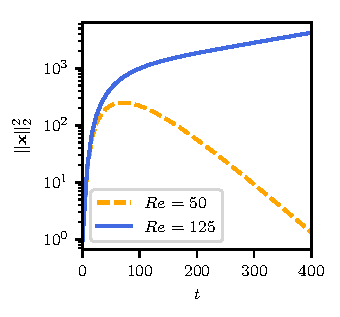
\includegraphics[scale=1]{S2_Theory_illustration_linear_stability}
    \caption{Evolution as a function of time of $\| \mathbf{x} \|_2^2 = x_1^2 + x_2^2$ for the toy-model \eqref{eq: theory -- schmid system}. For $Re=50$ (resp. $Re=125$), the asymptotic fate of $\| \mathbf{x} \|_2^2$ is described by a decreasing (resp. increasing) exponential. For $Re=50$, the equilibrium point is thus linear stable, while it is linearly unstable for $Re=125$.}
    \label{fig: theory -- illustration modal stability}
  \end{figure}

  %%%%%%%%%%%%%%%%%%%%%%%%%%%%%%%%%%%%%%%%%%%%%%%%
  %%%%%                                      %%%%%
  %%%%%     NON-MODAL STABILITY ANALYSIS     %%%%%
  %%%%%                                      %%%%%
  %%%%%%%%%%%%%%%%%%%%%%%%%%%%%%%%%%%%%%%%%%%%%%%%

  \subsection{Non-modal stability analysis}
  \label{subsec: theory -- non-modal stability}

  Looking once more at figure \ref{fig: theory -- illustration modal stability}, it can be seen that, although the system is linearly stable for $Re=50$, the perturbation $\mathbf{x}$ can experience a transient growth of its energy for a short period of time, roughly given by $0 < t <100$ in the present case, before its eventual exponential decay. This behavior is related to the \emph{non-normality} of $\mathbfcal{A}$, i.e.\
  \begin{equation}
    \mathbfcal{A}^H \mathbfcal{A} \neq \mathbfcal{A} \mathbfcal{A}^H,
    \label{eq: theory -- non-normality equation}
  \end{equation}
  where $\mathbfcal{A}^H$ is the Hermitian (also known as the \emph{adjoint}) of $\mathbfcal{A}$. As a result of this non-normality, the eigenvectors of $\mathbfcal{A}$ do not form an orthonormal set of vectors\footnote{Note that the non-normality of $\mathbfcal{A}$ also implies that its right and left eigenvectors are different. As will be discussed in \textsection \ref{sec: application}, this observation may have large consequences in fluid dynamics, particularly when addressing the problems of optimal linear control and/or estimation of strongly non-parallel flows.}. The consequences of this non-orthogonality of the set of eigenvectors can be visualized on figure \ref{fig: theory -- illustration transient growth} where the trajectory stemming from a random unit-norm initial condition $\mathbf{x}_0$ is depicted in the phase plane of our toy-model \eqref{eq: theory -- schmid system}. The perturbation $\mathbf{x}(t)$ is first attracted toward the linear manifold associated to the least stable eigenvalue $\lambda_1$, causing in the process the transient growth of its energy by a factor 300. Once it reaches the vicinity of the linearly stable manifold, the perturbation eventually decays exponentially rapidly along this eigendirection of the fixed point. The next sections are devoted to the introduction of mathematical tools particularly useful to characterize phenomena resulting from this non-normality of $\mathbfcal{A}$, both in the time and frequency domains, when the fixed point considered is stable.

  \begin{figure}[b]
    \centering
    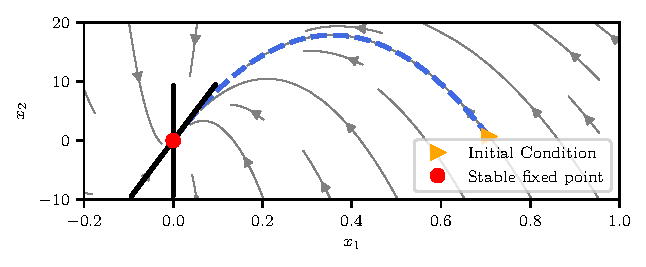
\includegraphics[scale=1]{S2_Theory_explanation_transient_growth}
    \caption{The blue (dashed) line shows the trajectory stemming from a random unit-norm initial condition $\mathbf{x}_0$. The thick black lines depict the two linear manifolds of the fixed point. The diagonal one corresponds to $\lambda_1 = \nicefrac{1}{100} - \nicefrac{1}{Re}$, while the vertical one is associated to $\lambda_2 = -\nicefrac{2}{Re}$. In the present case, $Re$ is set to 50, thus corresponding to a situation where the fixed point is linearly stable. Note that different scales are used for the horizontal and vertical axes.}
    \label{fig: theory -- illustration transient growth}
  \end{figure}

    %-----> Optimal perturbation.
    \subsubsection{Optimal perturbation analysis}
    \label{subsubsec: theory -- optimal perturbation}

    Having observed that a random initial condition can experience a relatively large transient growth of its energy over a short period of time even though the fixed point is stable, one may be interested in the worst case scenario, i.e.\ finding which initial condition $\mathbf{x}_0$ is amplified as much as possible before it eventually decays. Searching for such a perturbation is known as \emph{optimal perturbation analysis} and can be addressed by two different methods:
    \begin{itemize}
      \item Optimization,
      \item Singular Value Decomposition (SVD).
    \end{itemize}
    Both approaches will be presented. Although it requires the introduction of additional mathematical concepts, the approach relying on optimization will be introduced first in \textsection \ref{paragraph: theory -- optimal perturbation optimization} as it easier to grasp. The approach relying on singular value decomposition of the exponential propagrator $\mathbfcal{M} = \exp \left( \mathbfcal{A} t \right)$ will then be presented in \textsection \ref{paragraph: theory -- optimal perturbation svd}.

      % --> Lagrange multipliers.
      \paragraph{Formulation as an optimization problem}
      \label{paragraph: theory -- optimal perturbation optimization}

      The aim of optimal perturbation analysis is to find the unit-norm initial condition $\mathbf{x}_0$ that maximizes $\| \mathbf{x}(T) \|_2^2$, where $T$ is known as the \emph{target time}. Note that we here consider only the 2-norm of $\mathbf{x}(T)$ for the sake of simplicity, although one could formally optimize different norms, see \cite{??} for examples from fluid dynamics. For a given target time $T$, such a problem can be formulated as the following constrained maximization problem
      \begin{equation}
          \begin{aligned}
            \maximize \limits_{\mathbf{x}_0} & \mathcal{J} \left( \mathbf{x}_0 \right) = \| \mathbf{x}(T) \|_2^2\\
            \subjecto & \int_0^T \left( \dot{\mathbf{x}} - \mathbfcal{A}\mathbf{x} \right) \ \mathrm{d}t = 0 \\
            ~ & \| \mathbf{x}_0 \|_2^2 - 1 = 0,
          \end{aligned}
          \label{eq: theory -- constrained maximization}
      \end{equation}
      where $\mathcal{J}(\mathbf{x}_{0})$ is known as the \emph{objective function}. It must be emphasized that problem \eqref{eq: theory -- constrained maximization} is not formulated as a convex optimization problem\footnote{
      Formally, a convex optimization problem reads
      \begin{equation}
        \begin{aligned}
          \minimize \limits_{\mathbf{x}} & \mathcal{J} \left( \mathbf{x} \right) \\
          \subjecto & g_i \left( \mathbf{x} \right) \leq 0, \ i = 1, \cdots, m \\
          ~ & h_i \left( \mathbf{x} \right) = 0, \ i = 1, \cdots, p,
        \end{aligned}
        \notag
      \end{equation}
      where the objective function $\mathcal{J} \left( \mathbf{x} \right)$ and the inequality constraints functions $g_i \left( \mathbf{x} \right)$ are convex. The conditions on the equality constraints functions $h_i \left( \mathbf{x} \right)$ are more restrictive as they need to be affine functions, i.e.\ of the form $h_i \left( \mathbf{x} \right) = \mathbf{a}_i^T \mathbf{x} + b_i$. See the book by Boyd \& Vandenberghe \cite{book:boyd:2004} for extensive details about convex optimization.}.
      As such, it may exhibit local maxima. Nonetheless, this constrained maximization problem can be recast into the following unconstrained maximization problem
      \begin{equation}
        \maximize \limits_{\mathbf{x}, \mathbf{v}, \mu} \mathcal{L} \left( \mathbf{x}, \mathbf{v}, \mu \right),
        \label{eq: theory -- unconstrained maximization}
      \end{equation}
      where
      \begin{equation}
        \mathcal{L} \left( \mathbf{x}, \mathbf{v}, \mu \right) = \mathcal{J}\left( \mathbf{x}_0 \right) + \int_{0}^T \mathbf{v}^T \left( \dot{\mathbf{x}} - \mathbfcal{A}\mathbf{x} \right) \mathrm{d}t + \mu \left( \| \mathbf{x}_0 \|_2^2 - 1 \right)
        \label{eq: theory -- augmented Lagrangian}
      \end{equation}
      is known as the \emph{augmented Lagrangian} function. The additional optimization variables $\mathbf{v}$ and $\mu$ appearing in the definition of the augmented Lagrangian $\mathcal{L}$ are called \emph{Lagrange multipliers}. Solutions to problem \eqref{eq: theory -- unconstrained maximization} are identified by vanishing first variations of $\mathcal{L}$ with respect to our three optimization variables. The first variation of $\mathcal{L}$ with respect to $\mathbf{v}$ and $\mu$ are simply the constraints of our original problem \eqref{eq: theory -- constrained maximization}. The first variation of $\mathcal{L}$ with respect to $\mathbf{x}$ on the other hand is given by
      \begin{equation}
        \mathbf{0} = \left[ \nabla_{\mathbf{x}} \mathcal{J} + \mathbf{v}(T) \right] \cdot \delta \mathbf{x}(0) + \int_0^T \left[ \dot{\mathbf{v}} - \mathbfcal{A}^H \mathbf{v} \right] \cdot \delta \mathbf{x} \ \mathrm{dt} + \left[ 2\mu \mathbf{x}_0 - \mathbf{v}(0) \right] \cdot \delta \mathbf{x}(0).
        \label{eq: theory -- optimality condition}
      \end{equation}
      Eq. \eqref{eq: theory -- optimality condition} vanishes only if
      \begin{equation}
        \dot{\mathbf{v}} = \mathbfcal{A}^H \mathbf{v} \ \text{ over } t \in \left( 0, T \right),
        \label{eq: theory -- adjoint equations}
      \end{equation}
      and
      \begin{equation}
        \begin{aligned}
          \nabla_{\mathbf{x}} \mathcal{J} - \mathbf{v}(T) & = 0 \\
          2\mu \mathbf{x}_0 - \mathbf{v}(0) & = 0.
        \end{aligned}
        \label{eq: theory -- compatibility conditions}
      \end{equation}
      Note that Eq. \eqref{eq: theory -- adjoint equations} is known as the adjoint system\footnote{
      Given an appropriate norm, here the 2-norm, the adjoint operator $\mathbfcal{A}^H$ is defined such that
      \begin{equation}
        \langle \mathbf{v} \vert \mathbfcal{A} \mathbf{x} \rangle = \langle \mathbfcal{A}^H \mathbf{v} \vert \mathbf{x} \rangle,
        \notag
      \end{equation}
      where $\langle \mathbf{a} \vert \mathbf{b} \rangle$ is the standard Euclidean inner product in the present case.
      }
      of our original linear dynamical system, while Eq. \eqref{eq: theory -- compatibility conditions} are called compatibility conditions. Maximizing $\mathcal{L}$ is then a problem of simultaneously satisfying \eqref{eq: theory -- linear perturbation dynamics}, \eqref{eq: theory -- adjoint equations} and \eqref{eq: theory -- compatibility conditions}. This is in general done iteratively by gradient-based algorithms such as gradient descent or the rotation-update gradient algorithm (see \textsection \ref{sec: numerics}). For more details about adjoint-based optimization, see \cite{book:boyd:2004, nonlinear_optimal:kerswell:2014}.

      %--> A Rayleigh quotient problem.
      \paragraph{Formulation using SVD}
      \label{paragraph: theory -- optimal perturbation svd}

      As stated previously, formulating the optimal perturbation analysis as a constrained maximization results in a non-convex optimization problem \eqref{eq: theory -- constrained maximization}. Consequently, although a solution to \eqref{eq: theory -- constrained maximization} can easily be obtained by means of gradient-based algorithms, one cannot rule out the possibility that this solution is not the optimal one but only a local maxima. In this section, we will show that recasting problem \eqref{eq: theory -- constrained maximization} in the framework of linear algebra however allows us to obtain easily this global optimal.

      Let us first redefine our optimization problem as
      \begin{equation}
        \maximize_{\mathbf{x}_0} \displaystyle \frac{\| \mathbf{x}(T) \|_2^2}{\| \mathbf{x}_0 \|_2^2}
        \label{eq: theory -- energy gain}
      \end{equation}
      so that rather than maximizing $\| \mathbf{x}(T) \|_2^2$ under the constraint that $\| \mathbf{x}_0 \|_2^2 = 1$, we now directly aim to maximize the energy gain $\mathcal{G}(T) = \nicefrac{\| \mathbf{x}(T) \|_2^2}{\| \mathbf{x}_0 \|_2^2}$. Moreover, recalling from \eqref{eq: theory -- linear stability solution} that
      \begin{equation}
        \mathbf{x}(T) = \exp \left( \mathbfcal{A} T \right) \mathbf{x}_0,
        \notag
      \end{equation}
      our energy gain maximization problem can finally be written as
      \begin{equation}
        \begin{aligned}
          \mathcal{G}(T) & = \max_{\mathbf{x}_0} \displaystyle \frac{\| \exp \left( \mathbfcal{A} t \right) \mathbf{x}_0 \|_2^2}{\| \mathbf{x}_0 \|_2^2} \\
          & = \| \exp \left( \mathbfcal{A} T \right) \|_2^2
        \end{aligned}
      \end{equation}
      where $\| \exp \left( \mathbfcal{A} T \right) \|_2$ is a vector-induced matrix norm taking care of the optimization over all possible initial conditions $\mathbf{x}_0$. Introducing singular value decomposition (SVD), i.e.\
      \begin{equation}
        \mathbfcal{M} = \mathbfcal{U} \boldsymbol{\Sigma} \mathbfcal{V}^H,
        \notag
      \end{equation}
      it is relatively easy to demonstrate that the optimal energy gain $\mathcal{G}(T)$ is given by
      \begin{equation}
        \mathcal{G}(T) = \sigma_1^2,
        \label{theory -- optimal energy gain }
      \end{equation}
      where $\sigma_1$ is the dominant singular value of the exponential propagator $\mathbfcal{M} = \exp \left( \mathbfcal{A} T \right)$. The optimal initial condition $\mathbf{x}_0$ is then given by the principal right singular vector (i.e.\ $\mathbf{x}_0 = \mathbf{v}_1$), while the associated response is given by $\mathbf{x}(T) = \sigma_1 \mathbf{u}_1$, where $\mathbf{u}_1$ is the principal left singular vector.

      % --> Illustration.
      \paragraph{Illustration}

      {\color{red} Je pensais illustrer cette section en utilisant l'opérateur de Orr-Sommerfeld-Squire, sans pour autant rentrer dans les d\'etails des \'equations ni quoi que ce soit. Juste faire un cas (les streaks optimaux) et montrer la courbe de gain optimal, la perturbation initiale et la r\'eponse.}

    \subsubsection{Resolvent analysis}
    \label{subsubsec: theory -- resolvent perturbation}

    The optimal perturbation analysis (see \textsection \ref{subsubsec: theory -- optimal perturbation}) aims at finding the initial condition $\mathbf{x}_0$ that maximizes the transient amplification of energy of the response $\mathbf{x}(T) = \exp \left( \mathbfcal{A} T \right) \mathbf{x}_0$ at the target time $t=T$. It is thus an initial-value problem that can be investigated in the time domain. Rather than considering the response of the system to different initial conditions, one may instead wonder how the system reacts to external noise. For that purpose, let us now consider a forced linear dynamical system
    \begin{equation}
      \dot{\mathbf{x}} = \mathbfcal{A} \mathbf{x} + \mathbf{f}
      \label{eq: theory -- forced linear system}
    \end{equation}
    where the forcing $\mathbf{f}$ now models the system's input such as the external noise. As before, we moreover assume that all of the eigenvalues of $\mathbfcal{A}$ lie within the stable half of the complex plane. As for the optimal perturbation analysis, one may now consider a worst-case scenario, i.e.\ what is the forcing $\mathbf{f}$ that maximizes the asymptotic response of the system? Because we consider a linear dynamical system, this question can naturally be addressed in the frequency domain.

    In the most general case, the response of the system to the forcing $\mathbf{f}(t)$ is given by
    \begin{equation}
      \mathbf{x}(t) = \int_0^t \exp \left( \mathbfcal{A} (t-\tau) \right) \mathbf{f}(\tau) \ \mathrm{d}\tau
      \label{eq: theory -- convolution integral}
    \end{equation}
    which is a convolution integral. Note that, in the above expression, we assumed a zero initial condition, i.e.\ $\mathbf{x}_0 = 0$. Such a convolution integral is also known as a memory integral and highlights that the current state $\mathbf{x}(t)$ of the system depends on the entire history of the forcing $\mathbf{f}$. Because we consider linear stable systems, the influence of the forcing on the current state decays exponentially according to the least stable eigenvalue. Let us assume furthermore a harmonic external forcing
    \begin{equation}
      \mathbf{f}(t) = \Re \left( \hat{\mathbf{f}} e^{i \omega t} \right)
    \end{equation}
    where $\omega \in \mathbb{R}$ is the forcing circular frequency. The convolution integral can now be easily computed in the frequency domain. Given our assumptions, the asymptotic response of the system at the frequency $\omega$ is given by
    \begin{equation}
      \hat{\mathbf{x}} = \left( i \omega \mathbfcal{I} - \mathbfcal{A} \right)^{-1} \hat{\mathbf{f}}.
      \label{eq: theory -- transfer function}
    \end{equation}
    The operator $\mathbfcal{R}(\omega) = \left( i \omega \mathbfcal{I} - \mathbfcal{A} \right)^{-1}$ appearing in Eq. \eqref{eq: theory -- transfer function} is known as the \emph{Resolvent operator} and is related to the exponential propagator $\mathbfcal{M}(t) = \exp \left( \mathbfcal{A} t \right)$ via Laplace transform. This operator, acting in the frequency domain, maps the input harmonic forcing $\hat{\mathbf{f}}(\omega)$ to the output harmonic response $\hat{\mathbf{x}}(\omega)$.

    Finding the forcing frequency $\omega$ that maximizes the asymptotic response $\mathbf{x}$ of the system can now be formalized as
    \begin{equation}
      \begin{aligned}
        \mathcal{R}(\omega) & = \max_{\hat{\mathbf{f}}} \displaystyle \frac{\| \left( i \omega \mathbfcal{I} - \mathbfcal{A} \right)^{-1} \hat{\mathbf{f}} \|_2^2}{\| \hat{\mathbf{f}} \|_2^2} \\
        & = \| \mathbfcal{R}(\omega) \|_2^2.
      \end{aligned}
      \label{eq: theory -- resolvent norm}
    \end{equation}
    Going from the time domain to the frequency domain, the norm of the exponential propagator is replaced with that of the resolvent in order quantify the energy amplification between the input forcing and the output response. As before, the optimal resolvent gain at the frequency $\omega$ is given by
    \begin{equation}
      \mathcal{R}(\omega) = \sigma_1^2,
      \notag
    \end{equation}
    where $\sigma_1$ is the leading singular value of $\mathbfcal{R}(\omega)$. The associated optimal forcing $\hat{\mathbf{f}}$ and response $\hat{\mathbf{x}}$ are then given by the corresponding right and left singular vectors, respectively.

    % --> Illustration.
    \paragraph{Illustration}

    {\color{red} Pareil que pour la perturbation optimale.}


% --> Numerical methods.
\section{Numerical methods}
\label{sec: numerics}

In this section, different techniques will be presented to solve modal and non-modal stability problems for very large-scale dynamical systems. Such very large-scale systems typically arise from the spatial discretization of partial differential equations, e.g.\ the Navier-Stokes equations in fluid dynamics. Throughout this section, the two-dimensional shear-driven cavity flow at various Reynolds numbers will serve as an example. The same configuration as \cite{??} is considered. The dynamics of the flow are governed by
\begin{equation}
  \begin{aligned}
    \displaystyle \frac{\partial \mathbf{U}}{\partial t} + \left( \mathbf{U} \cdot \nabla \right) \mathbf{U} & = - \nabla P + \frac{1}{Re} \nabla^2 \mathbf{U} \\
    \nabla \cdot \mathbf{U} & = 0,
  \end{aligned}
  \label{eq: numerics -- Navier-Stokes equations}
\end{equation}
where $\mathbf{U}$ is the velocity field and $P$ is the pressure field. Figure \ref{fig: numerics -- shear-driven cavity flow} depicts a typical vorticity snapshot obtained from direct numerical simulation at a supercritical Reynolds number.

Given a fixed point $\mathbf{U}_b$ of the Navier-Stokes equations \eqref{eq: numerics -- Navier-Stokes equations}, the dynamics of an infinitesimal perturbation $\mathbf{u}$ evolving on top of it are governed by
\begin{equation}
  \begin{aligned}
    \displaystyle \frac{\partial \mathbf{u}}{\partial t} + \left( \mathbf{u} \cdot \nabla \right) \mathbf{U}_b  + \left( \mathbf{U}_b \cdot \nabla \right) \mathbf{u} & = - \nabla p + \frac{1}{Re} \nabla^2 \mathbf{u} \\
    \nabla \cdot \mathbf{u} & = 0.
  \end{aligned}
  \label{eq: numerics -- linearized Navier-Stokes equations}
\end{equation}
Once projected onto a divergence-free vector space, Eq. \eqref{eq: numerics -- linearized Navier-Stokes equations} can be formally written as
\begin{equation}
  \dot{\mathbf{u}} = \mathbfcal{A}\mathbf{u},
  \label{eq: numerics -- linearized Navier-Stokes equations bis}
\end{equation}
where $\mathbfcal{A}$ is the linearized Navier-Stokes operator. After being discretized in space, $\mathbfcal{A}$ is a $n \times n$ matrix. For our example, the computational domain is discretized using ??? grid points, resulting in a total of $2 \times ??$ degrees of freedom. From a practical point of view, explicitly assembling the resulting matrix $\mathbfcal{A}$ would require approximately ?? Gb. Investigating the stability properties of this two-dimensional flow would thus not be possible on a simple laptop at the moment despite the simplicity of the case considered. It has to be noted however that, given an initial condition $\mathbf{u}_0$, the analytical solution to Eq. \eqref{eq: numerics -- linearized Navier-Stokes equations bis} reads
\begin{equation}
  \mathbf{u}(T) = \exp \left( \mathbfcal{A}T \right) \mathbf{u}_0,
  \notag
\end{equation}
where $\mathbfcal{M} = \exp \left( \mathbfcal{A}T \right)$ is the exponential propagator introduced previously. Although assembling explicitly this matrix $\mathbfcal{M}$ is even harder than assembling $\mathbfcal{A}$, its application onto the vector $\mathbf{u}_0$ can easily be computed using a classical time-stepping code solving the linearized Navier-Stokes equations \eqref{eq: numerics -- linearized Navier-Stokes equations}. Such a \emph{time-stepper} approach has been popularized by \cite{??}. In the rest of this section, the different algorithms proposed for fixed point computation, linear stability and non-modal stability analyses will heavily rely on this time-stepper strategy. The key point is that they require only minor modifications of an existing time-stepping code to be put into use.

  %%%%%%%%%%%%%%%%%%%%%%%%%%%%%%%%%%%%%%%%%%%%%%%%%%%%%%%
  %%%%%                                             %%%%%
  %%%%%     KRYLOV METHODS FOR LINEAR EQUATIONS     %%%%%
  %%%%%                                             %%%%%
  %%%%%%%%%%%%%%%%%%%%%%%%%%%%%%%%%%%%%%%%%%%%%%%%%%%%%%%

  % \subsection{Krylov methods for for solving linear systems}
  % \label{subsubsec: theory -- krylov methods}



  %%%%%%%%%%%%%%%%%%%%%%%%%%%%%%%%
  %%%%%                      %%%%%
  %%%%%     FIXED POINTS     %%%%%
  %%%%%                      %%%%%
  %%%%%%%%%%%%%%%%%%%%%%%%%%%%%%%%

  \subsection{Fixed points computation}
  \label{subsec: numerics-fixed points computation}

  The starting point when investigating a nonlinear dynamical system it to determine its fixed points. As discussed in \textsection \ref{subsec: theory-fixed points}, for a continuous-time dynamical system, such points are solution to
  \begin{equation}
    \mathbfcal{F} \left( \mathbf{X} \right) = 0,
    \label{eq: numerics -- continuous-time fixed point}
  \end{equation}
  while one needs to solve
  \begin{equation}
    \mathbf{X} - \mathbfcal{G} \left( \mathbf{X} \right) = 0
    \label{eq: numerics -- discrete-time fixed point}
  \end{equation}
  for a discrete-time nonlinear dynamical system. In this section, three different fixed point solvers will be presented.

    %-----> Selective frequency damping.
    \subsubsection{Selective Frequency Damping}
    \label{subsubsec: numerics -- selective frequency damping}

    Selective frequency damping is a fixed point computation technique proposed by {\AA}kervik \emph{et al.}\ \cite{pof:akervik:2006} in 2006 and largely adapted from the original work of Pruett \emph{et al.}\ \cite{pof:pruett:2003, pof:pruett:2006} on temporal approximate deconvolution models for large-eddy simulations. It has since become one of the standard approaches for fixed point computation in fluid dynamics due to its ease of implementation. Note that various implementations of the original selective frequency damping method have been proposed over the years \cite{pof:jordi:2014, pof:jordi:2015, pof:cunha:2015}. Moreover, it has since been extented to compute steady states of the Reynolds-Averaged-Navier-Stokes (RANS) equations \cite{cf:richez:2016} as well as for the computation of unstable periodic orbits \cite{prf:leopold:2017}. In the rest of this section, only the original formulation by {\AA}kervik \emph{et al.}\ \cite{pof:akervik:2006} will be described.

    Let us consider a fixed point $\mathbf{X}^*$ of the nonlinear system
    $$\dot{\mathbf{X}} = \mathbfcal{F} \left( \mathbf{X} \right).$$
    If $\mathbf{X}^*$ is linearly unstable, then any initial condition $\mathbf{X}_0 \neq \mathbf{X}^*$ will quickly depart from $\mathbf{X}^*$. Using standard regularization techniques from control theory, the aim of selective frequency damping is thus to stabilize the linearly unstable fixed point $\mathbf{X}^*$. For that purpose, one can use proportional feedback control so that the forced system now reads
    \begin{equation}
      \dot{\mathbf{X}} = \mathbfcal{F} \left( \mathbf{X} \right) - \chi \left( \mathbf{X} - \mathbf{Y} \right),
      \label{eq: numerics -- sfd forced system}
    \end{equation}
    where $\chi$ is the control gain and $\mathbf{Y}$ the target solution. This target solution is obviously the fixed point one aims to stabilize, i.e.\ $\mathbf{Y} = \mathbf{X}^*$, which is unfortunately not known \emph{a priori}. It has to be noted however that, for a large range of situations, the instability of the fixed point $\mathbf{X}^*$ will tend to give rise to unsteady dynamics. In such cases, the target solution $\mathbf{Y}$ is thus a modification of $\mathbf{X}$ with \emph{reduced temporal fluctuations}, i.e.\ a temporally low-pass filtered solution. This filtered solution is defined as
    \begin{equation}
      \mathbf{Y}(t) = \mathcal{H}(t, \Delta) * \mathbf{X}(t-\tau)
      \label{eq: numerics -- low-pass filtered solution}
    \end{equation}
    where $\mathcal{H}$ is the convolution kernel of the applied causal low-pass filter and $\Delta$ the filter witdh. Using such definitions, the forced system \eqref{eq: numerics -- sfd forced system} can thus be rewritten as
    \begin{equation}
      \dot{\mathbf{X}} = \mathbfcal{F}\left( \mathbf{X} \right) - \chi \left( \mathbfcal{I} - \mathcal{H} \right) * \mathbf{X}.
      \label{eq: numerics -- sfd foced system bis}
    \end{equation}
    As $\mathbf{X}$ tends to the fixed point $\mathbf{X}^*$, the low-pass filtered solution $\mathbf{Y}$ tends to $\mathbf{X}$. Once a steady state has been reached, one has
    $$\mathbf{X} = \mathbf{Y} = \mathbf{X}^*,$$
    i.e.\ the fixed point of the controlled system \eqref{eq: numerics -- sfd foced system bis} is the same as that of our original system. Moreover, as the system approaches its fixed point, the amplitude of the proportional feedback control term vanishes.

    \paragraph{Applying the low-pass filter in the time domain}

    As it is formulated, computing the low-pass filtered solution \eqref{eq: numerics -- low-pass filtered solution} requires the evaluation of the following convolution integral
    \begin{equation}
      \mathbf{Y}(t) = \int_{-\infty}^t \mathcal{H}(\tau-t, \Delta) \mathbf{X}(\tau) \mathrm{d}\tau.
      \label{eq: numerics -- convolution integral}
    \end{equation}
    Note that, to be admissible, the kernel $\mathcal{H}$ must be positive and properly normalized. Moreover, in the limit of vanishing filter width, it must approach the Dirac delta function. To the best of our knowledge, all implementations of the selective frequency damping thus relies on the exponential kernel
    \begin{equation}
      \mathcal{H}(\tau - t, \Delta) = \displaystyle \frac{1}{\Delta} \exp \left( \frac{\tau - t}{\Delta} \right).
      \label{eq: numerics -- exponential kernel}
    \end{equation}
    The corresponding Laplace transform is given by
    \begin{equation}
      \hat{\mathcal{H}}(\omega, \Delta) = \displaystyle \frac{1}{1 + i \omega \Delta}.
      \label{eq: numerics -- laplace transform}
    \end{equation}
    The cutoff frequency of this filter is given by $\omega_c = \nicefrac{1}{\Delta}$. Figure \ref{fig: numerics -- lapalce transform} depicts the real part of $\hat{\mathcal{H}}$ as a function of the frequency $\omega$ for $\Delta=1$. Naturally, this cutoff frequency needs to be tuned so that the frequency associated to the instability one aims to kill is quenched by the filter.

    For real applications, evaluating the convolution integral \eqref{eq: numerics -- convolution integral} is impractical as it necessitates the storage of the complete time history of $\mathbf{X}$. Consequently, it is replaced by its differential form given by
    \begin{equation}
      \dot{\mathbf{Y}} = \displaystyle \frac{1}{\Delta} \left( \mathbf{X} - \mathbf{Y} \right)
      \label{eq: numerics -- differential filter formulation}
    \end{equation}
    which can be integrated in time using classical integration schemes, e.g.\ second-order backward Euler. Combining \eqref{eq: numerics -- differential filter formulation} and \eqref{eq: numerics -- sfd forced system} finally yields to the following extended system
    \begin{equation}
      \left\{
      \begin{aligned}
        \dot{\mathbf{X}} & = \mathbfcal{F}\left( \mathbf{X} \right) - \chi \left( \mathbf{X} - \mathbf{Y} \right) \\
        \dot{\mathbf{Y}} & = \displaystyle \frac{1}{\Delta} \left( \mathbf{X} - \mathbf{Y} \right).
      \end{aligned}
      \right.
      \label{eq: numerics -- selective frequency damping}
    \end{equation}
    Implementing \eqref{eq: numerics -- selective frequency damping} into an existing time-stepping code requires only minor modifications, hence making it an easy choice for fixed point computation. It must be emphasized however that, because it relies on a low-pass filtering procedure, this selective frequency damping method is unable to quench non-oscillating instabilities, e.g.\ instabilities arising due to a pitchfork bifurcation. This particular point is one of its major limitations.

    \begin{figure}[b]
      \sidecaption
      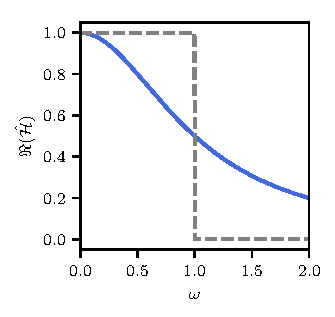
\includegraphics[scale=1]{S3_SFD_transfer_function}
      \caption{Evolution of $\Re \left( \hat{\mathcal{H}} \right)$ ({\color{blue} ---}), i.e.\ the real part of the Laplace transform of the exponential filter, as a function of the frequency $\omega$ for $\Delta=1$. The gray dashed line depicts the ideal spectral cutoff filter.}
      \label{fig: numerics -- lapalce transform}
    \end{figure}

    %-----> Newton-Krylov method.
    \subsubsection{Newton-Krylov methods}
    \label{subsubsec: numerics -- newton-krylov methods}

    While we relied on the continuous time representation of our system in \textsection \ref{subsubsec: numerics -- selective frequency damping}, we will now turn to its discrete-time counterpart in order to stay as close as possible to the actual time-stepper implementation of the algorithm to be describe. For that purpose, we will thus consider the following nonlinear system
    \begin{equation}
      \mathbf{X}_{k+1} = \mathbfcal{G}\left( \mathbf{X}_k \right).
      \label{eq: numerics -- discrete time system}
    \end{equation}
    Our goal is thus to find a fixed point $\mathbf{X}$ of this problem. Newton-Raphson method is a natural choice, provided the dimension of $\mathbf{X}$ is not too large. For large-scale dynamical systems, one may turn to the class of Newton-Krylov methods instead. These encompasses a wide variety of different approaches, part of which have been reviewed in \cite{jcp:knoll:2004}. In the rest of this section, we will present a variant of the recursive projection method originally proposed by Shroff \& Keller \cite{siam:shroff:1993}.

    % It can be shown that iteration \eqref{eq: numerics -- discrete time system} converges if all the eigenvalues $\{ \mu_k \}_1^n$ of the Jacobian of $\mathbfcal{G}$ lie in the unit disk and the initial iterate $\mathbf{X}_0$ is sufficiently close to the actual fixed point $\mathbf{X}^*$. Note moreover that, for our purposes, the Jacobian of $\mathbfcal{G}$ is given by the exponential propagator
    % \begin{equation}
    %   \mathbfcal{M} = \exp \left( \mathbfcal{A} T \right).
    %   \label{eq: numerics -- jacobian matrix}
    % \end{equation}
    % Iteration \eqref{eq: numerics -- discrete time system} will however fail to converge if any eigenvalues of $\mathbfcal{M}$ lies outside the unit disk. Moreover, if all eigenvalues are within the unit disk, convergence may be slow if any of them lie close to the boundary of the disk.

    %-----> BoostConv.
    \subsubsection{BoostConv}

    %-----> Comparison.
    \subsubsection{Comparison of the different approaches}


  %%%%%%%%%%%%%%%%%%%%%%%%%%%%%%%%%%%%%%%%%%%%
  %%%%%                                  %%%%%
  %%%%%     MODAL STABILITY ANALYSIS     %%%%%
  %%%%%                                  %%%%%
  %%%%%%%%%%%%%%%%%%%%%%%%%%%%%%%%%%%%%%%%%%%%

  \subsection{Linear stability and eigenvalue computation}

  The aim of linear stability analysis is to determine whether a perturbation $\textbf{x}$, governed by
  \begin{equation}
    \dot{ \mathbf{x} } = \mathbfcal{A} \mathbf{x},
    \notag
  \end{equation}
  will grow or decay exponentially rapidly as $t \to \infty$. This asymptotic behavior is entirely governed by the eigenspectrum of the Jacobian matrix $\mathbfcal{A}$: if at least one of its eigenvalues has a positive (resp. negative) real part, the linear system considered is unstable (resp. stable), see \textsection \ref{subsec: theory -- linear stability} for more details.

  It must emphasized that, within a time-stepper framework, one does not seek directly for the eigenpairs of the Jacobian matrix $\mathbfcal{A}$ of the continuous-time problem. Instead, the problem considered is recast in the discrete-time framework as
  \begin{equation}
    \mathbf{x}_{k+1} = \mathbfcal{M} \mathbf{x}_k,
    \label{eq: numerics -- discrete-time linear system}
  \end{equation}
  where $\mathbfcal{M} = \exp \left( \mathbfcal{A} T \right)$ is the exponential propagator already introduced in \textsection \ref{subsec: theory -- linear stability}, \textsection \ref{subsubsec: theory -- optimal perturbation}, and \textsection \ref{subsubsec: numerics -- newton-krylov methods}, and where $T$ is the sampling period. The system is then linearly unstable if at least one eigenvalue $\mu$ of $\mathbfcal{M}$ lies outside the unit disk, i.e. $\vert \mu \vert > 1$.

  As discussed previously, although one cannot explicitly assemble the exponential propagator $\mathbfcal{M}$, its action onto a given vector $\mathbf{x}_k$ simply amounts to march in time the linearized system from $t = kT$ to $t = (k+1)T$. This ability to evaluate relatively easily the matrix-vector product given by \eqref{eq: numerics -- discrete-time linear system} allows us to use iterative solvers as to compute the eigenpairs of $\mathbfcal{M}$. The rest of this section is thus devoted to the presentation of two iterative eigenvalue solvers, namely the Arnoldi decomposition and the Krylov-Schur decomposition.
    % %-----> Power Iteration.
    % \subsubsection{Power Iteration method}
    % \label{subsubsec: numerics -- power iteration}

    %-----> Arnoldi decomposition.
    \subsubsection{Arnoldi decomposition}
    \label{subsubsec: numerics -- arnoldi}

    Let us denote the following sequence of vectors
    \begin{equation}
      \mathbfcal{K}_m\left( \mathbfcal{M}, \mathbf{v}_0 \right) = \left\{ \mathbf{v}_0, \mathbfcal{M}\mathbf{v}_0, \cdots, \mathbfcal{M}^{m-1} \mathbf{v}_0 \right\}.
      \label{eq: numerics -- krylov sequence}
    \end{equation}
    Eq. \eqref{eq: numerics -- krylov sequence} is known as a \emph{Krylov sequence} eventually converging toward the eigenvector associated to the largest eigenvalue (in modulus) of $\mathbfcal{M}$ as $m \to \infty$. Generating this sequence to approximate the leading eigenpair of $\mathbfcal{M}$ is known as the \emph{power iteration method}. Note that this simple method retains only the last vector of this sequence while discarding the information contained in the first $m-1$ vectors.

    Contrary to the power iteration method, Arnoldi decomposition uses all of the information contained in the Krylov sequence \eqref{eq: numerics -- krylov sequence} as to compute better estimates of the leading eigenvalues of $\mathbfcal{M}$. Readers can easily be convinced that the Krylov sequence \eqref{eq: numerics -- krylov sequence} obeys
    \begin{equation}
      \mathbfcal{M} \mathbfcal{K}_m \simeq \mathbfcal{K}_m \mathbfcal{C},
      \notag
    \end{equation}
    where $\mathbfcal{C}$ is a $m \times m$ companion matrix representing the low-dimensional projection of $\mathbfcal{M}$ onto the span of the Krylov sequence \eqref{eq: numerics -- krylov sequence}. As such, the eigenpairs of $\mathbfcal{C}$ approximate the leading eigenpairs of $\mathbfcal{M}$. It must be emphasized however that, as $m$ increases, the last vectors in the Krylov sequence become almost parallel. Consequently, the companion matrix $\mathbfcal{C}$ becomes increasingly ill-conditioned. As to overcome the loss of information from the power iteration method and the increasingly ill-conditioned companion matrix decomposition, the Arnoldi method combines them with a Gram-Schmidt orthogonalization process. The basic Arnoldi iteration then reads
    \begin{equation}
      \mathbfcal{MV}_m = \mathbfcal{V}_m \mathbfcal{H}_m + \mathbf{r}_{m} \mathbf{e}^T_m,
      \label{eq: numerics -- m-step Arnoldi}
    \end{equation}
    where $\mathbfcal{V}_m$ is an orthonormal set of vectors, $\mathbfcal{H}_m$ is a $m \times m$ upper Hessenberg matrix and $\vert \mathbf{r}_{m} \mathbf{e}^T_m \vert$ is the residual indicating how far $\mathbfcal{V}_m$ is from from an invariant subspace of $\mathbfcal{M}$. Because of its relatively small dimension, the eigenpairs $\left( \mu_H, \mathbf{y} \right)$ of the Hessenberg matrix, also known as Ritz pairs, can be computed using direct eigensolvers, e.g.\ QZ decomposition. The Ritz pairs of $\mathbfcal{H}_m$ are related to the eigenpairs of $\mathbfcal{M}$ as follows
    \begin{equation}
      \begin{aligned}
        \mu_{\mathbfcal{M}} & \simeq \mu_{\mathbfcal{H}} \\
        \hat{\mathbf{u}} & \simeq \mathbfcal{V}_m \mathbf{y}.
      \end{aligned}
    \end{equation}
    A detailed presentation of the basic $m$-step Arnoldi factorization is given in algorithm \eqref{algo: Arnoldi} while figure \ref{fig: numerics -- arnoldi decomposition} depicts its block-diagram representation to ease the understanding. As can be seen, Arnoldi decomposition is relatively simple to implement within an existing time-stepper code. One has to bear in mind however that this technique resembles some sophisticated signal processing. As a consequence, in order to capture (within a time-stepper framework) an eigenpair of the Jacobian matrix $\mathbfcal{A}$ characterized by a circular frequency $\omega$, one has to obey the Nyquist criterion and needs at least four snapshots to appropriately discretize the associated period.

    \begin{algorithm}
      \begin{algorithmic}
        \REQUIRE $\mathbfcal{M} \in \mathbb{R}^{n \times n}$, starting vector $\mathbf{v} \in \mathbb{R}^n$.\\
        $\mathbf{v}_1 = \mathbf{v} / \| \mathbf{v} \|$;\\
        $\mathbf{w} = \mathbfcal{M} \mathbf{v}_1$; \\
        $\alpha_1 = \mathbf{v}_1^T \mathbf{w}$;\\
        $\mathbf{f}_1 \leftarrow \mathbf{w} - \alpha_1 \mathbf{v}_1$;\\
        $\mathbfcal{V}_1 \leftarrow \left( \mathbf{v}_1 \right)$; \\
        $\mathbfcal{H}_1 \leftarrow (\alpha_1)$;\\
        \FOR{$j=1,2,\cdots,m-1$}
        \STATE{$\beta_j=\|\mathbf{f}_j\|$; \\
        $\mathbf{v}_{j+1} \leftarrow \mathbf{f}_j/\beta_j$; \\
        $\mathbfcal{V}_{j+1} \leftarrow \left( \mathbfcal{V}_j, \mathbf{v}_{j+1} \right)$;\\

        $\hat{\mathbfcal{H}}_j \leftarrow \begin{pmatrix}
                                            \mathbfcal{H}_j \\
                                            \beta_j \mathbf{e}_j^T
                                          \end{pmatrix}
        $ \\
        $\mathbf{w} \leftarrow \mathbfcal{M} \mathbf{v}_{j+1}$;\\
        $\mathbf{h} \leftarrow \mathbfcal{V}_{j+1}^T \mathbf{w}$; \\
        $\mathbf{f}_{j+1} \leftarrow \mathbf{w} - \mathbfcal{V}_{j+1} \mathbf{h}$;\\
        $\mathbfcal{H}_{j+1} \leftarrow (\hat{\mathbfcal{H}}_j,\mathbf{h})$;}
        \ENDFOR
      \end{algorithmic}
      \caption{The $m$-step \emph{Arnoldi} factorisation.}
      \label{algo: Arnoldi}
    \end{algorithm}

    \begin{figure}[b]
      \centering
      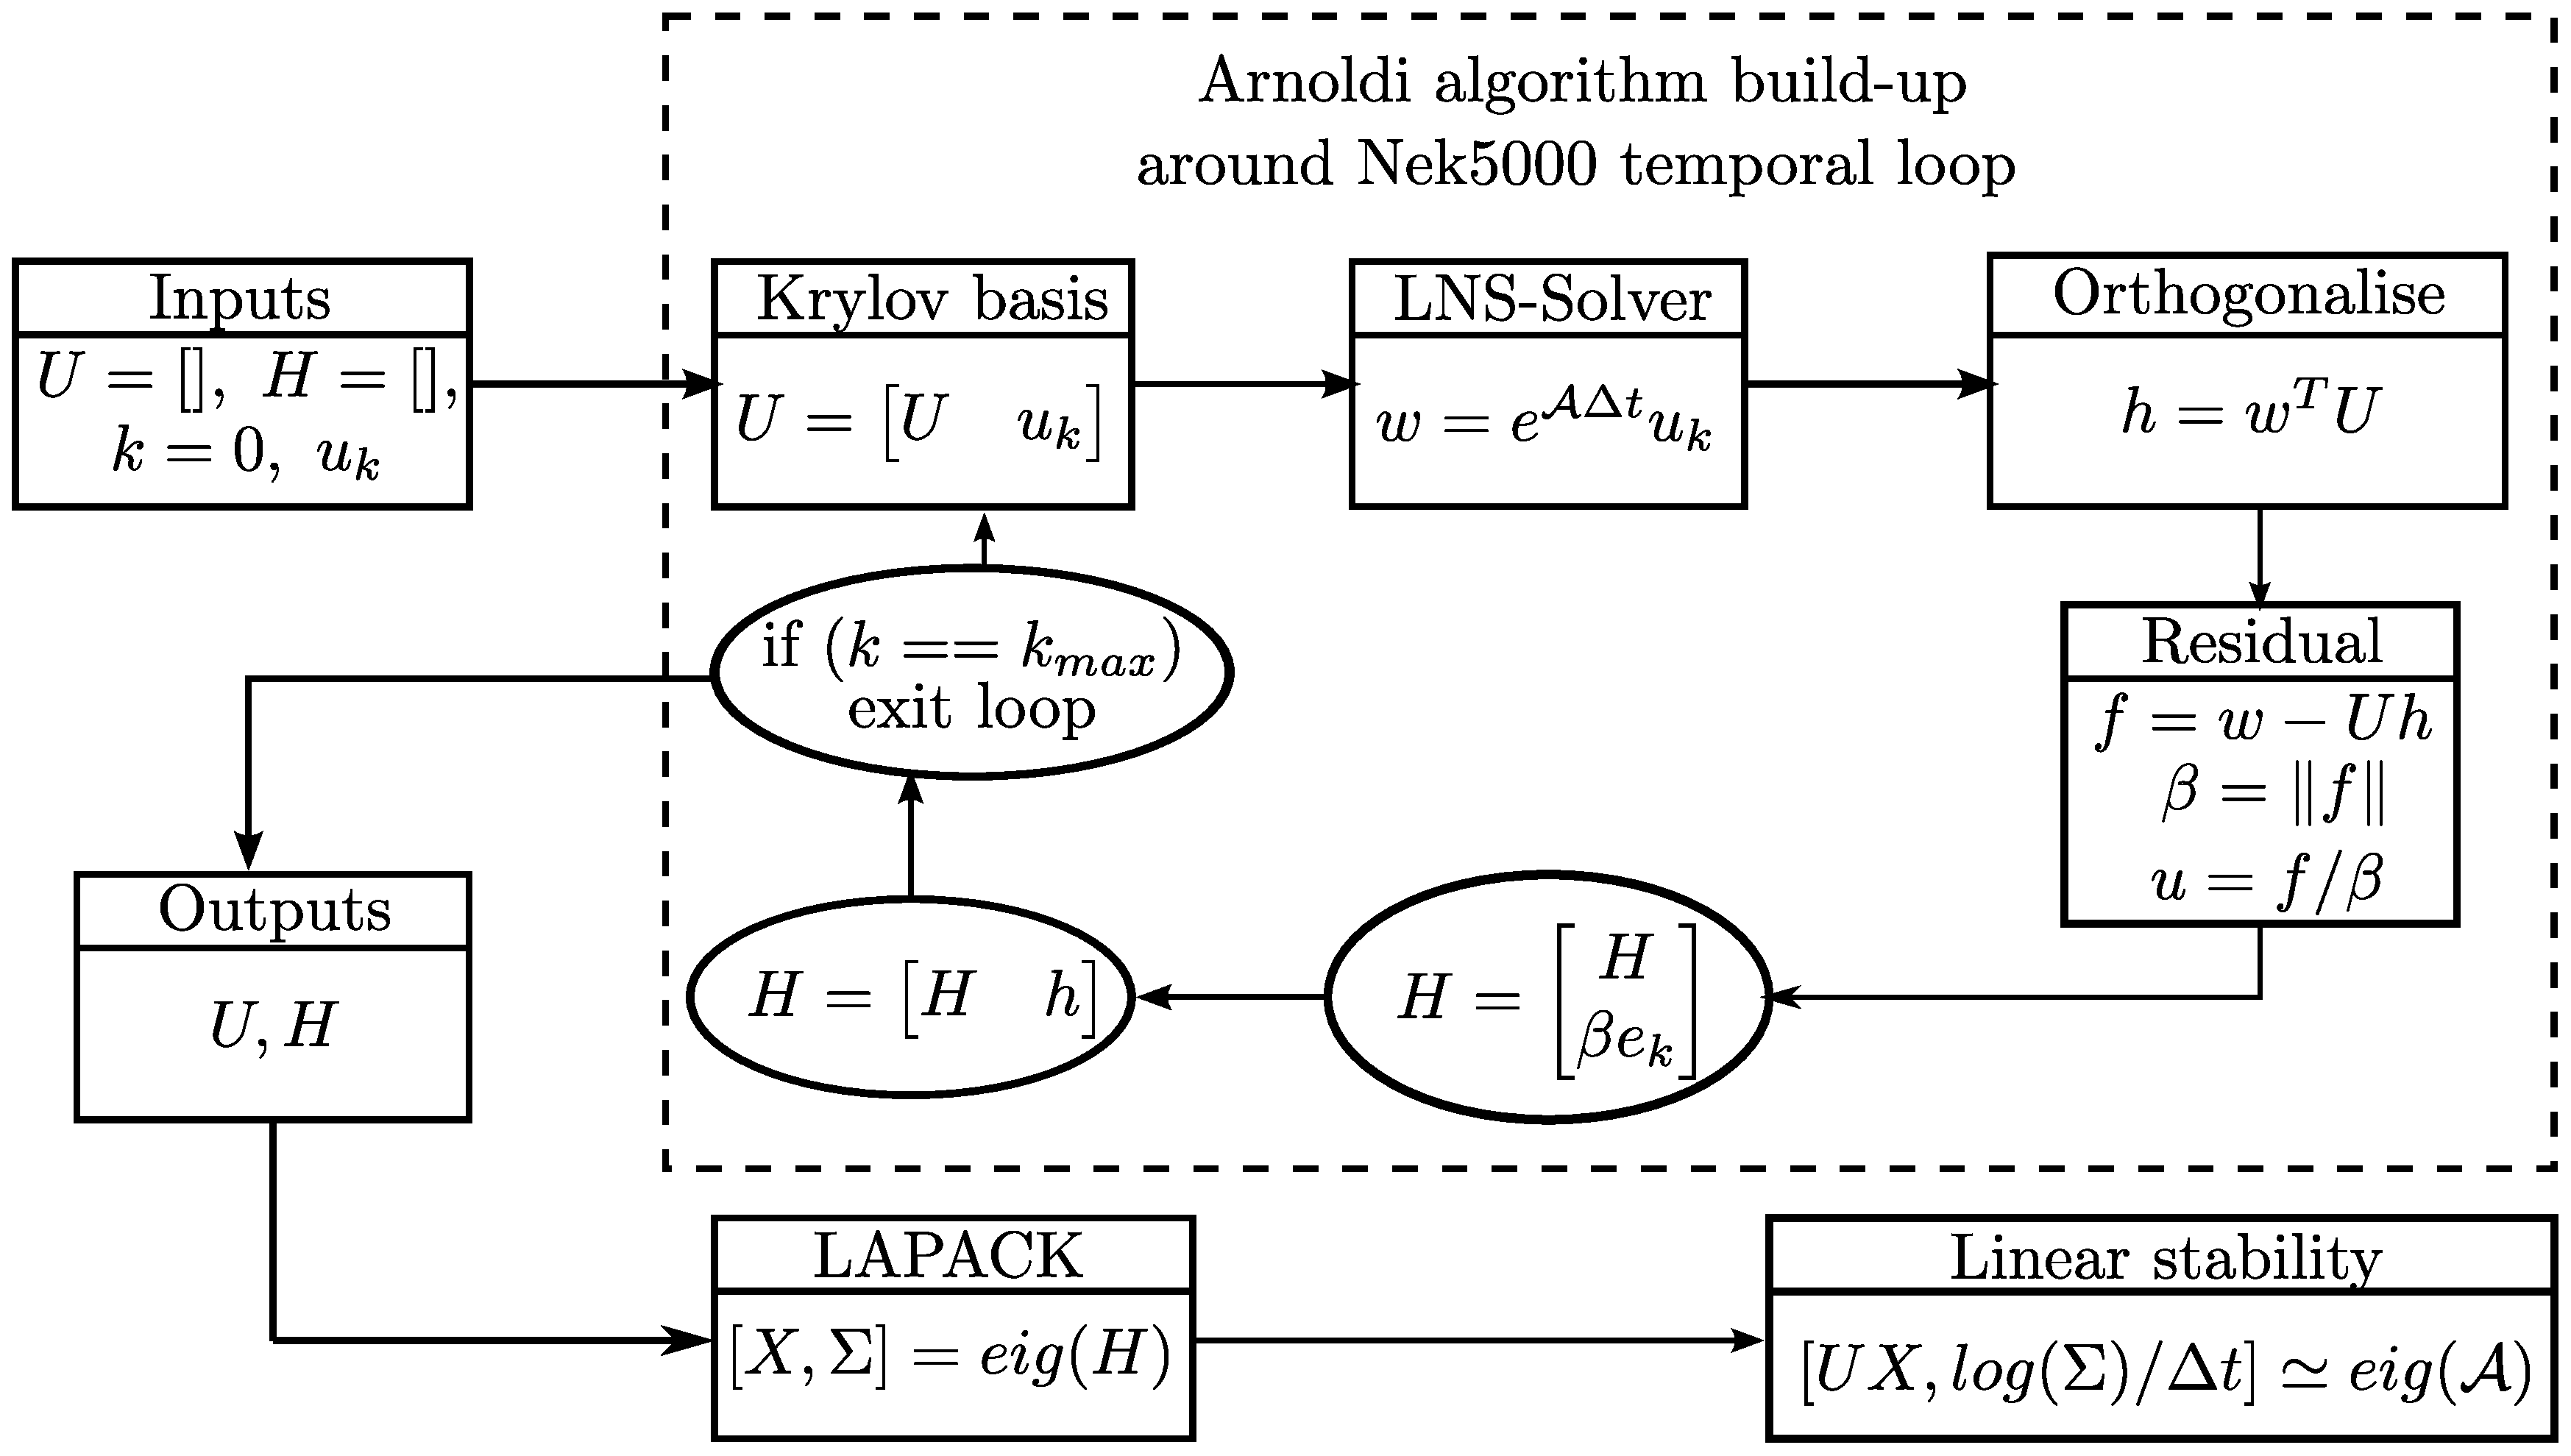
\includegraphics[width=.9\textwidth]{Arnoldi}
      \caption{Block-diagram representation of the basic $m$-step Arnoldi factorization. Note that, within a time-stepper framework, every matrix-vector product $\mathbfcal{M} \mathbf{v}_i$ is evaluated by marching in time the linearized system considered.}
      \label{fig: numerics -- arnoldi decomposition}
    \end{figure}

    %-----> Krylov-Schur decomposition.
    \subsubsection{Krylov-Schur decomposition}

    Let us consider the $m$-step Arnoldi factorization
    \begin{equation}
      \mathbfcal{MV}_m = \mathbfcal{V}_m \mathbfcal{H}_m + \beta \mathbf{v}_{m+1} \mathbf{e}^T_m
      \label{eq: m-step Arnoldi}
    \end{equation}
    introduced in \textsection \ref{subsubsec: numerics -- arnoldi}. As discussed previously, the Ritz pair $\left( \mu_H, \mathbfcal{V}_m \mathbf{y} \right)$ of $\mathbfcal{H}_m$ provides a good approximation for the eigenpair $\left( \mu, \hat{\mathbf u} \right)$ of the matrix $\mathbfcal{M}$. One limitation of the Arnoldi decomposition is however that the dimension $m$ of the Krylov subspace necessary to converge the leading Ritz pairs is not known \emph{a priori}. It might hence be relatively large, thus potentially causing some numerical and/or practical problems (e.g.\ storage of Krylov basis $\mathbfcal{V}_m$, forward instability of the Gram-Schmidt process involved in the Arnoldi decomposition, etc). Two different approaches have been proposed to overcome these limitations: the \emph{Implicitly Restarted Arnoldi Method} introduced by Sorensen \cite{Sorensen_SIAM_1992} in 1992 and the \emph{Krylov-Schur decomposition} introduced by Stewart \cite{Stewart_SIAM_2001} in 2001. In the present work, the latter approach has been preferred because of its simplicity of implementation and its robustness.

    The Krylov-Schur method is based on the generalization of the m-step Arnoldi factorization~\eqref{eq: m-step Arnoldi} to a \emph{Krylov decomposition} of order $m$
    \begin{equation}
      \mathbfcal{MV}_m = \mathbfcal{V}_m \mathbfcal{B}_m + \mathbf{v}_{m+1} \mathbf{b}_{m+1}^T
      \label{eq: Krylov decomposition}
    \end{equation}
    in which the matrix $\mathbfcal{B}_m$ and the vector $\mathbf{b}_{m+1}$ have no restriction. The Arnoldi decomposition then appears as a special case of Krylov decomposition when $\mathbfcal{B}_m$ is restricted to be in upper Hessenberg form and $\mathbf{b}_{m+1} = \mathbf{e}_m$. Another special case is the \emph{Krylov-Schur} decomposition in which the matrix $\mathbfcal{B}_m$ is in real Schur form (i.e.\ quasi-triangular form with its eigenvalues in the $1 \times 1$ or $2 \times 2$ diagonal blocks). It has been shown by Stewart \cite{Stewart_SIAM_2001} that Krylov and Arnoldi decompositions are equivalent (i.e.\ they have the same Ritz approximations). Moreover, by means of orthogonal similarity transformations, any Krylov decomposition can be transformed into an equivalent Krylov-Schur decomposition. The core of the Krylov-Schur method is thus based on a two-steps procedure: (\emph{i}) an expansion step performed using a $m$-step Arnoldi factorization, and (\emph{ii}) a contraction step to a Krylov-Schur decomposition of order $p$ retaining only the most useful spectral information from the initial $m$-step Arnoldi decomposition. Given an initial unit-norm vector $\mathbf{v}_1$, a subroutine to compute the matrix-vector product $\mathbfcal{M} \mathbf{v}_i$, and the desired dimension $m$ of the Krylov subspace, the Krylov-Schur method can be summarized as follows:
    \begin{enumerate}
      \item Construct an initial Krylov decomposition of order $m$ using for instance the $m$-step Arnoldi factorization~\eqref{eq: m-step Arnoldi}.

      \item Check for the convergence of the Ritz eigenpairs. If a sufficient number has converged, then stop. Otherwise, proceed to step 3.

      \item Compute the real Schur decomposition $\mathbfcal{B}_m = \mathbfcal{Q} \mathbfcal{S}_m \mathbfcal{Q}^T$ such that the matrix $\mathbfcal{S}_m$ is in real Schur form and $\mathbfcal{Q}$ is the associated matrix of Schur vectors. It is assumed furthermore that the Ritz values on the diagonal blocks of $\mathbfcal{S}_m$ have been sorted such that the $p$ ''wanted'' Ritz values are in the upper-left corner of $\mathbfcal{S}_m$, while the $m-p$ ''unwanted'' ones are in the lower-right corner. At this point, we have the following re-ordered Krylov-Schur decomposition
      \begin{equation}
        \mathbfcal{M} \tilde{\mathbfcal{V}}_m =
        \tilde{\mathbfcal{V}}_m
        \begin{bmatrix}
         \mathbfcal{S}_{11} & \mathbfcal{S}_{12} \\
         {\mathbf 0}     & \mathbfcal{S}_{22}
       \end{bmatrix}
       + {\mathbf v}_{m+1}\begin{bmatrix}
                           {\mathbf b}_{1}^T & {\mathbf b}_{2}^T
                           \end{bmatrix}
        \label{eq: Krylov-Schur decomposition}
      \end{equation}
      with $\tilde{\mathbfcal{V}}_m = \mathbfcal{V}_m  \mathbfcal{Q}$ being the re-ordered Krylov basis, $\mathbfcal{S}_{11}$ the subset of the Schur matrix containing the $p$ ''wanted'' Ritz values, $\mathbfcal{S}_{22}$ the subset containing the $m-p$ ''unwanted'' ones, and $\begin{bmatrix} {\mathbf b}_1^T & {\mathbf b}_2^T \end{bmatrix} = {\mathbf b}^T \mathbfcal{Q}$.

      \item Truncate the Krylov-Schur decomposition~\eqref{eq: Krylov-Schur decomposition} of order $m$ to a Krylov decomposition of order $p$,
        \begin{equation}
          \mathbfcal{M}\tilde{\mathbfcal{V}}_p = \tilde{\mathbfcal{V}}_p \mathbfcal{S}_{11} + \tilde{\mathbf v}_{p+1}{\mathbf b}_1^T
        \end{equation}
      with $\tilde{\mathbfcal{V}}_p$ equal to the first $p$ columns of $\tilde{\mathbfcal{V}}_m$ and $\tilde{\mathbf v}_{p+1} = {\mathbf v}_{m+1}$.

      \item Extend again to a Krylov decomposition of order $m$ using a variation of the procedure used in the first step: the procedure is re-initialized with the starting vector ${\mathbf v}_{p+1}$ but all the vectors in $\tilde{\mathbfcal{V}}_p$ are taken into account in the orthogonalization step.

      \item Check the convergence of the Ritz values. If not enough Ritz values have converged, restart from step 3.

    \end{enumerate}
    This algorithm has two critical steps. The first one is the choice of the ''wanted'' Ritz values in the re-ordering of the Schur decomposition in step 2. Since we are only interested in the leading eigenvalues of the linearized Navier-Stokes operator, all the Ritz pairs being classified as ''wanted'' must satisfy $\left| \mu_w \right| \ge 1 - \delta$ (with $\delta = 0.05 - 0.1$ usually). Regarding the criterion assessing the convergence of a given Ritz pair, starting from the Krylov decomposition~\eqref{eq: m-step Arnoldi}, one can write
    \begin{equation}
      \| \mathbfcal{M} \mathbfcal{V}_m \mathbf{y} - \mathbfcal{V}_m \mathbfcal{B}_m \mathbf{y} \| = \| \mathbfcal{M} \mathbfcal{V}_m \mathbf{y} - \mu_{\mathbf B} \mathbfcal{V}_m \mathbf{y} \| = \left| \beta \mathbf{e}_m^T \mathbf{y} \right|
      \label{eq: Krylov convergence}
    \end{equation}
    with $(\mu_{\mathbf B},\mathbf{y})$ a given eigenpair of the matrix $\mathbfcal{B}_m$. If the right hand side $\left| \beta {\mathbf e}_{m}^T{\mathbf y} \right|$ is smaller than a given tolerance, then the Ritz pair $(\mu_{\mathbf B}, \mathbfcal{V}_m {\mathbf y})$ provides a good approximation to the eigenpair $(\mu, \hat{\mathbf u})$ of the original matrix $\mathbfcal{M}$. A Ritz value is generally considered as being converged if the associated residual $\left| \beta {\mathbf e}_{m}^T{\mathbf y} \right| \le 10^{-6}$.

    %-----> Comparisons.
    \subsubsection{Comparison of the two approaches}

  %%%%%%%%%%%%%%%%%%%%%%%%%%%%%%%%%%%%%%%%%%%%%%%%
  %%%%%                                      %%%%%
  %%%%%     NON-MODAL STABILITY ANALYSIS     %%%%%
  %%%%%                                      %%%%%
  %%%%%%%%%%%%%%%%%%%%%%%%%%%%%%%%%%%%%%%%%%%%%%%%

  \subsection{Non-modal stability and singular value decomposition}

    %-----> Optimal perturbation.
    \subsubsection{Optimal perturbation analysis}

    %-----> Resolvent analysis.
    \subsubsection{Resolvent analysis}


% --> Applications.
\section{Application to fluid dynamics}
\label{sec: application}


% --> Conclusion and perspectives.
\section{Conclusions and perspectives}
\label{sec: conclusion}



\bibliography{bibliography}
\bibliographystyle{plain}

\end{document}
